\chapter{OpenStreetMap, the data source}

OpenStreetMap (OSM) is a collaborative community project creating a full, editable representation of our world. It was founded in 2004 by Steve Coast, and now boasts over ten million registered volunteer users providing data from around the globe. Unlike proprietary services (such as Google Maps or Apple Maps), OSM data is open and freely available to build on or modify.\cite{osmHistory}

\section{Why OpenStreetMap?}

As my intentions with this thesis project included following free and open source software guidelines (see~\ref{licensing}), OSM was a perfect match to allow for further potential derivate works. Its widespread use also makes it easy to find and import arbitrary cities' datasets into the program, practically removing the limit on the area covered.

The sheer amount of data stored on the platform can be difficult to comprehend; it can be used for historical city maps, viewing hiking trails or even indoor navigation. Because of the many contributors from different countries, it contains information only available to locals. It's usually up-to-date, thanks to easy to use uploading tools, such as the web editor iD or the mobile app StreetComplete (see figure~\ref{scee}).

\begin{figure}[h]
    \centering
    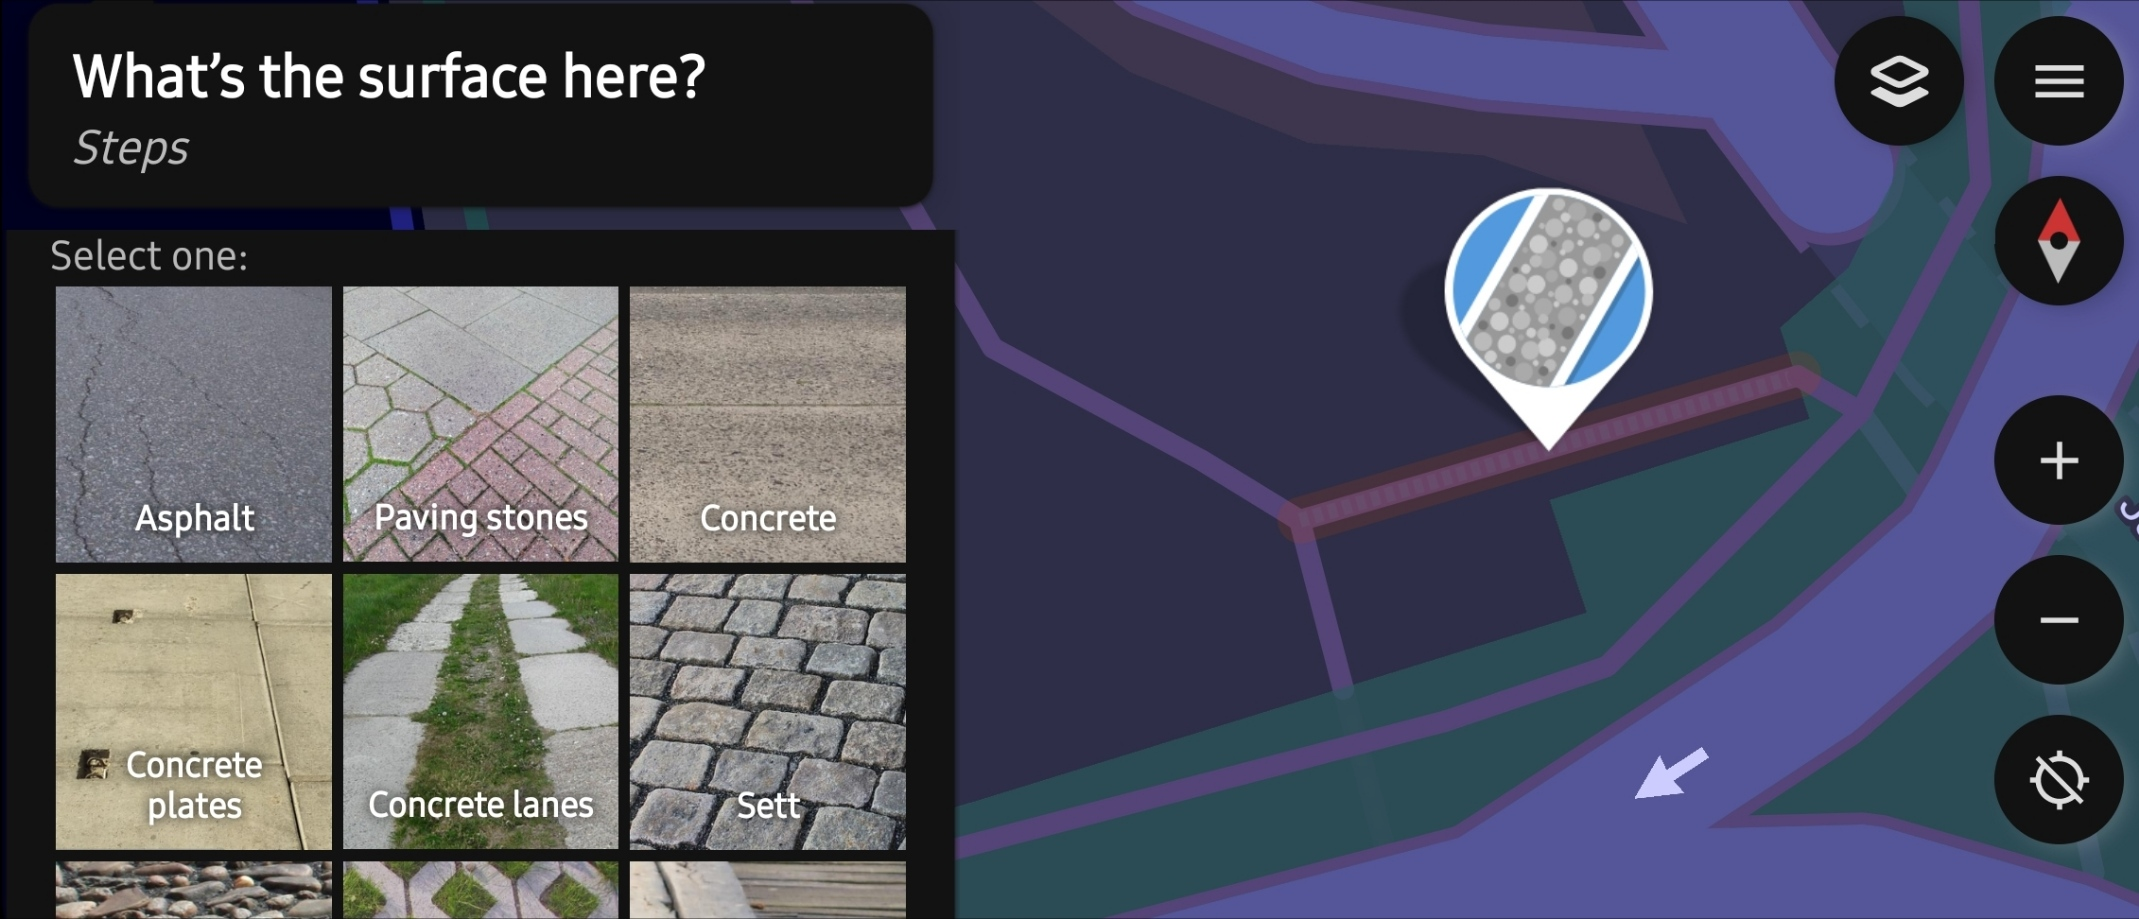
\includegraphics[width=140mm, keepaspectratio]{images/scee_example.jpg}
    \caption{A "quest" in the SCEE app, an improved version of StreetComplete; the user can submit information they see in real life \label{scee}}
\end{figure}

I also took a liking to discovering the mapping service powering most apps I use, and was interested in contributions to the dataset myself. Using it for my application would help me understand the inner workings better.

\section{Semantic data structure}

OpenStreetMap data is made up of elements -- nodes, ways and relations -- each describing some specific feature in space. Every element can contain multiple tags.~\cite{osmElements} Tags are simple key-value pairs which can store strings only, but may be used to represent complicated concepts. The meaning of each key is somewhat loosely defined and isn't standardised as there are over 96.000 of them -- guidelines do exist, however\footnote{\url{https://wiki.openstreetmap.org/wiki/Map_features}}. For example, they can range from \verb|name=Tüskesátor|, defining a simple building name, to \verb|source:maxspeed=HU:zone:30|, which details speed restrictions as applicable to the zone a given road is in.

The simplest element is a node. They represent objects that can only reasonably be represented as a single point, such as a bench or a newsstand. Over nine billion of these nodes exist, with 64-bit integer identification numbers and seven decimal places of precision for their latitude and longitude. Declaring elevation above sea level is optional.

A way can combine multiple nodes into a polyline, a connected chain of points. The accuracy can depend on the author, as there is no curve interpolation; the sparser the contained nodes are, the more jagged the way becomes. There are more than one billion ways, and they may be open (the last and first point is not connected) or closed. Buildings usually fall into the latter category.

Relations are catch-all elements and may represent anything more complex than a single way -- they're lists of nodes and ways with metadata added through tags. A complicated building may be treated as a relation, just as an intercity bus route is a connection of highways and streets. Child elements can have roles: for example, the main and side streams of a river.

With the gigantic userbase of OSM, guidelines for uploaded data are very important to ensure consistency. All information must be verifiable; the various mapping applications make it clear that one should only input data they confirmed in real life. Opinions, predictions and personal information are generally not allowed. Best practices also describe how buildings and roads -- the elements relevant to this app -- should be mapped.\cite{osmGoodPractices}

A building may be any of the three element types, with ways being most common. Whenever reasonable, the boundary of the building is defined as a single way. If there's a courtyard or other inner part that should be excluded, two ways are generally used as part of a multipolygon relation. The stated roles are almost always "inner" and "outer"; I chose "outer" wherever possible, to simplify looks. Buildings always have the \verb|building| tag and that can be used to attach a purpose to it: residential, commercial, industrial, public \etc. The project heavily relies on this tagging to filter the dataset, and the simulation would be nearly useless without it. The \verb|height| and \verb|levels| tags are optional but thankfully often used, giving the buildings a definite vertical size in metres and storeys respectively.

Roads and walkways of all kinds are OSM ways, identified with the \verb|highway| tag, which also categorises each road section (\eg primary, service, motorway). They're treated two dimensionally and stored as lines connecting multiple points. Highways are often grouped into junctions using a relation. The number of lanes, speed limits, and sidewalk state is also frequently tagged.


\section{Technical data structure}

Live online data is most easily queried through the Overpass API\footnote{\url{https://wiki.openstreetmap.org/wiki/Overpass_API}}. It provides read-only access to OSM elements and accepts a wide variety of filters. The returned information is JSON-convertible, making it ideal for apps that require more control than what pre-made web map plugins can provide. Queries use a custom language that simplifies searching by key and supports recursion well. The Overpass Turbo\footnote{\url{https://overpass-turbo.eu}} app has a wizard that helps with the correct syntax for Overpass requests.

Data is most often distributed in a heavily compressed Protocolbuffer Binary Format (PBF\footnote{\url{https://wiki.openstreetmap.org/wiki/PBF_Format}}) file. BBBike\footnote{\url{https://download.bbbike.org/osm}} provides exports of many large cities, as well as the ability to download a file containing information on a zone up to 6000 by 4000 kilometres large. On the scale of the entire planet, PBF saves over 96\% in storage space when compared to regular XML. PBF files utilise Google's Protocol Buffer\footnote{\url{https://github.com/protocolbuffers/protobuf}} interchange format. Based on a schema specification (not unlike one made for databases), a protocol buffer compiler can create low-level, efficient code for serialisation into said schema. Each \verb|.pbf| file is a series of binary blobs with headers, ultimately encoding key-value pairs in a string format. The obvious downside is that reading this data requires specialised libraries that can decode and uncompress it. I depended on osm4j\footnote{\url{https://github.com/topobyte/osm4j}} for this task, as it has a simple iterator to unpack elements sequentially. It's worth noting that PBF files store elements in the order of Node, Way, Relation. Relations and ways use foreign keys with a number format to connect to their child nodes.

OSM data may also be packaged in the XML format, which is much easier to read or edit as a user. However, even when compressed, it's about double the size of a PBF file. Due to its unoptimised nature, it's slower to parse and process.